\begin{figure}[h]
\centering
\textbf{Query}

\begin{tabular}{|p{0.7\linewidth}|}
\hline
What is the chemical formula for the ferroelectric material Lead Zirconium Titanate (PZT)? \\
\hline
\end{tabular}
\\
\textbf{Corpus}
\\
\begin{tabular}{|>{\centering\arraybackslash} p{0.7\linewidth}|}
\hline

\includegraphics[width=0.8\linewidth,frame]{figures/examples_assests/document_understanding/corpus_1.pdf} \\
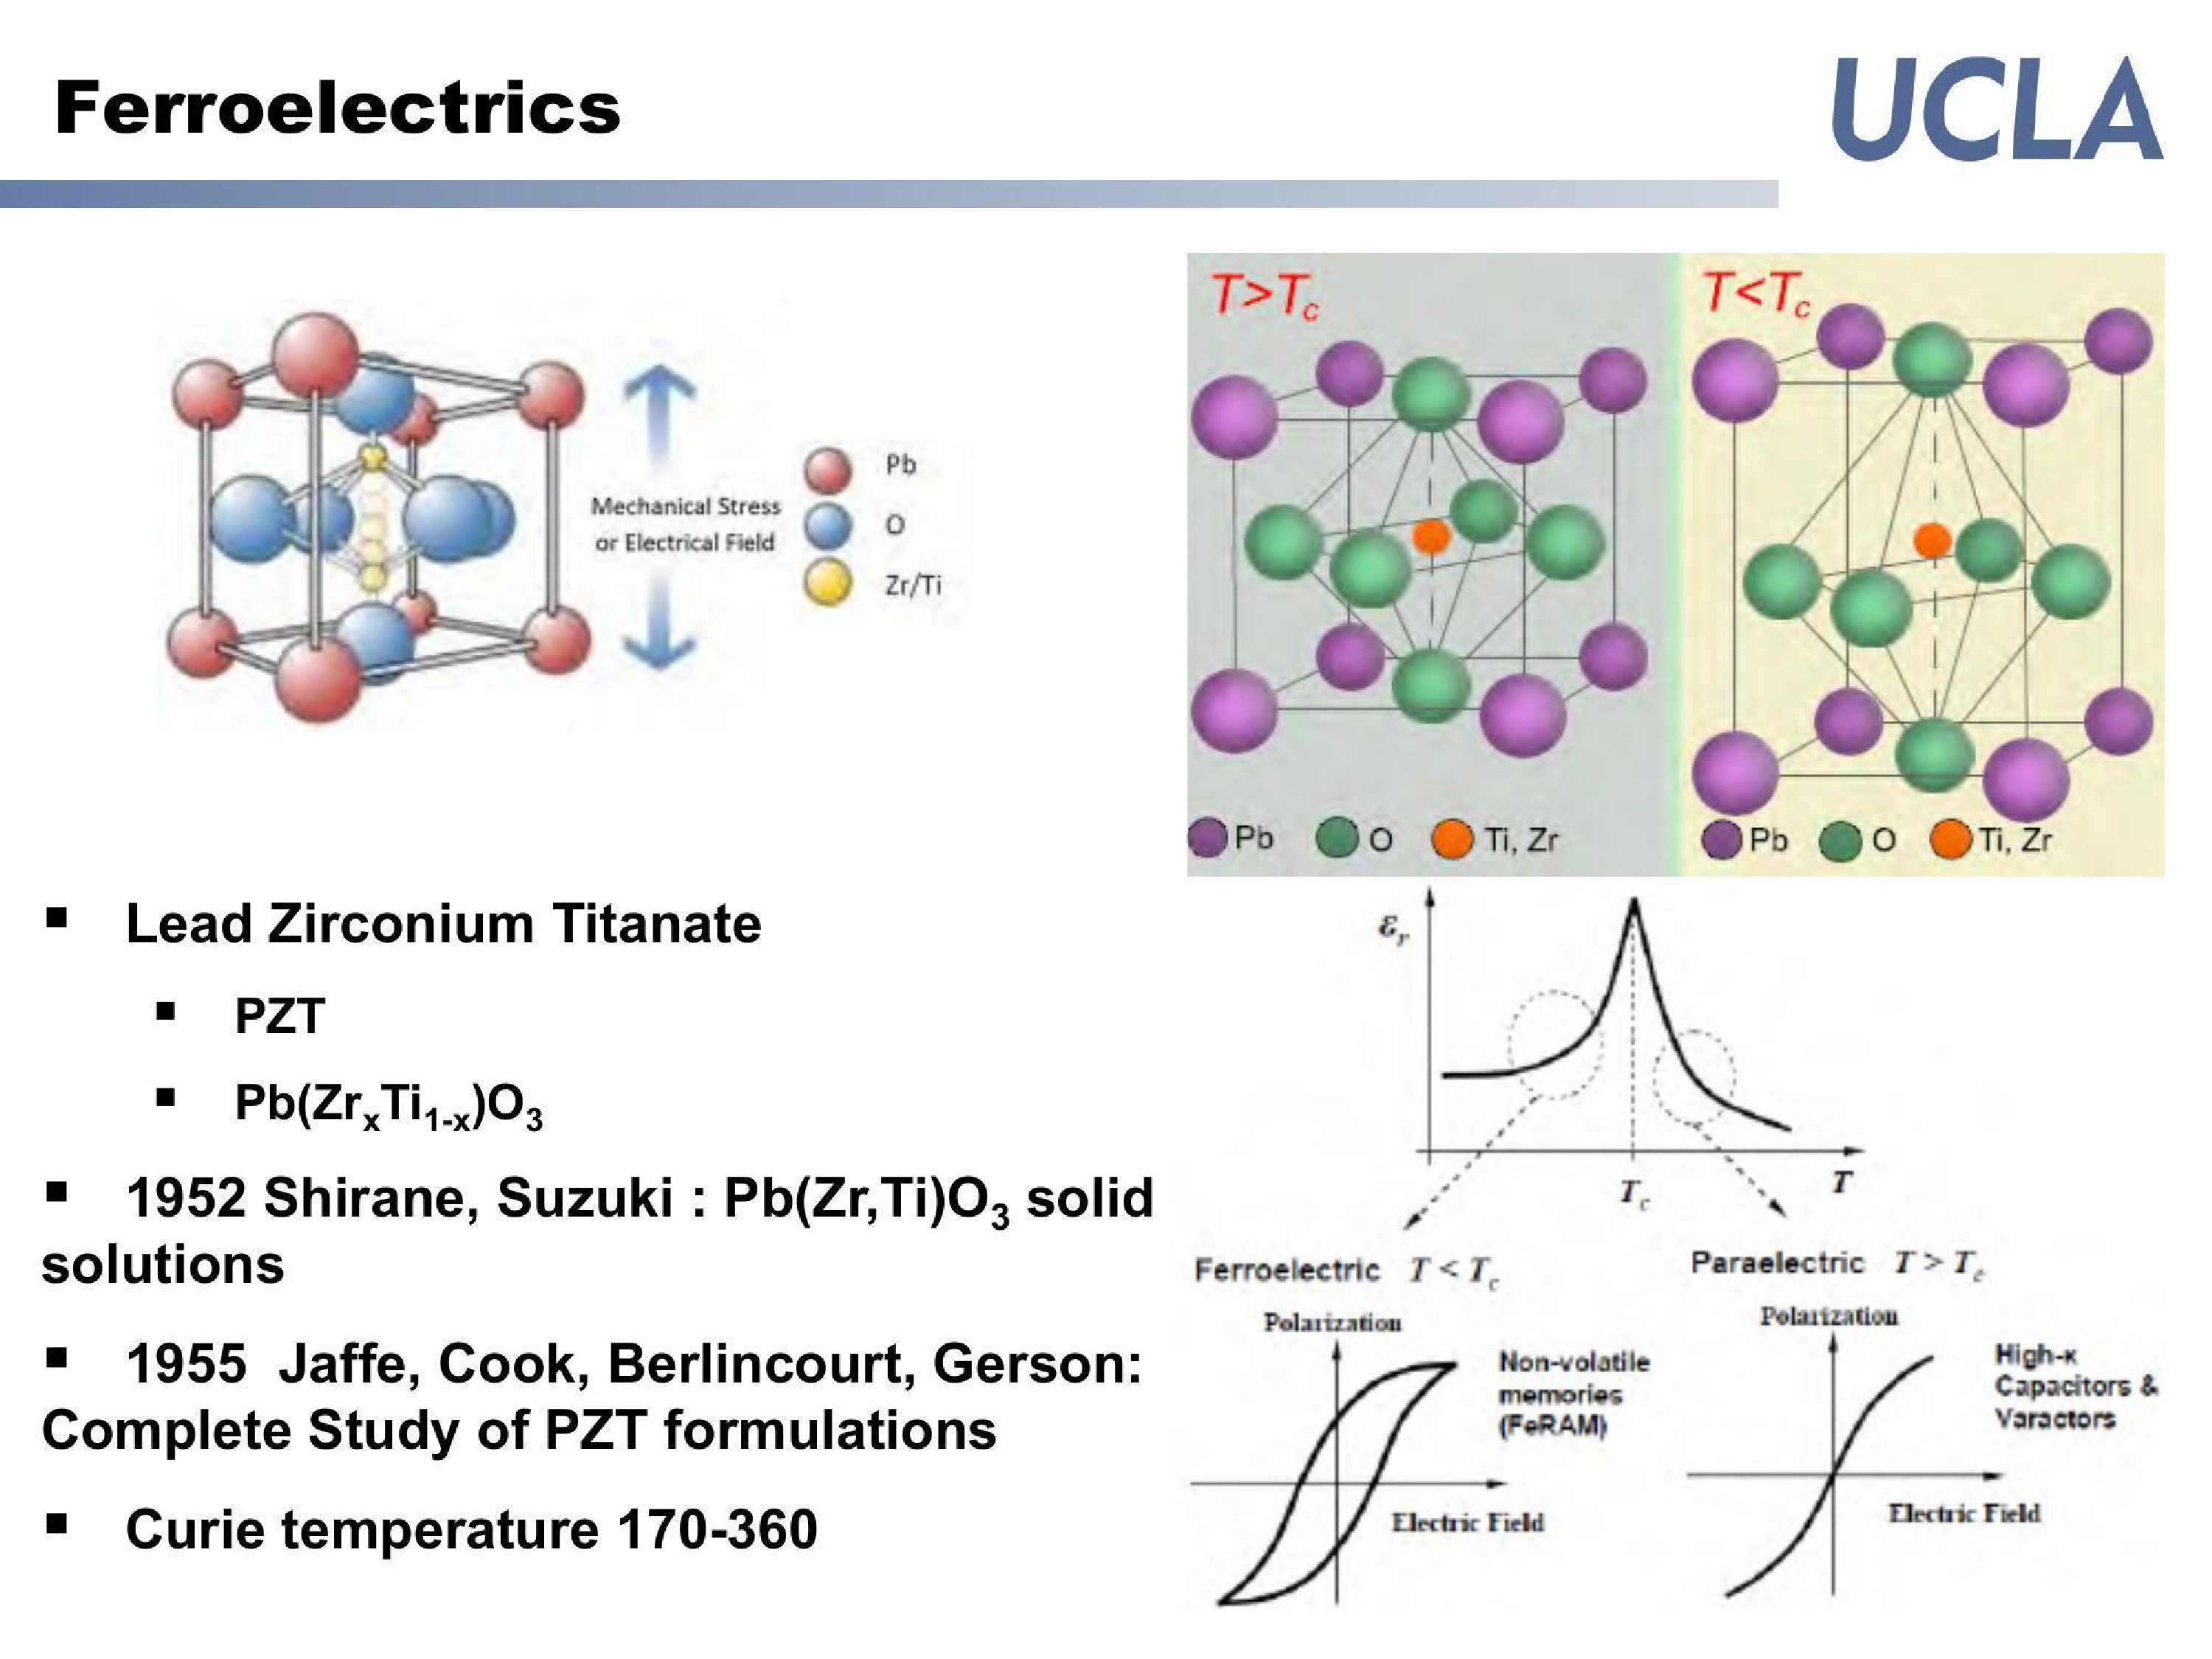
\includegraphics[width=0.8\linewidth,frame]{figures/examples_assests/document_understanding/answer.pdf} \\

\includegraphics[width=0.8\linewidth,frame]{figures/examples_assests/document_understanding/corpus_2.pdf} \\
\hline
\end{tabular}
\\
\textbf{Relevant document} 
\\
\begin{tabular}{|>{\centering\arraybackslash} p{0.7\linewidth}|}
\hline
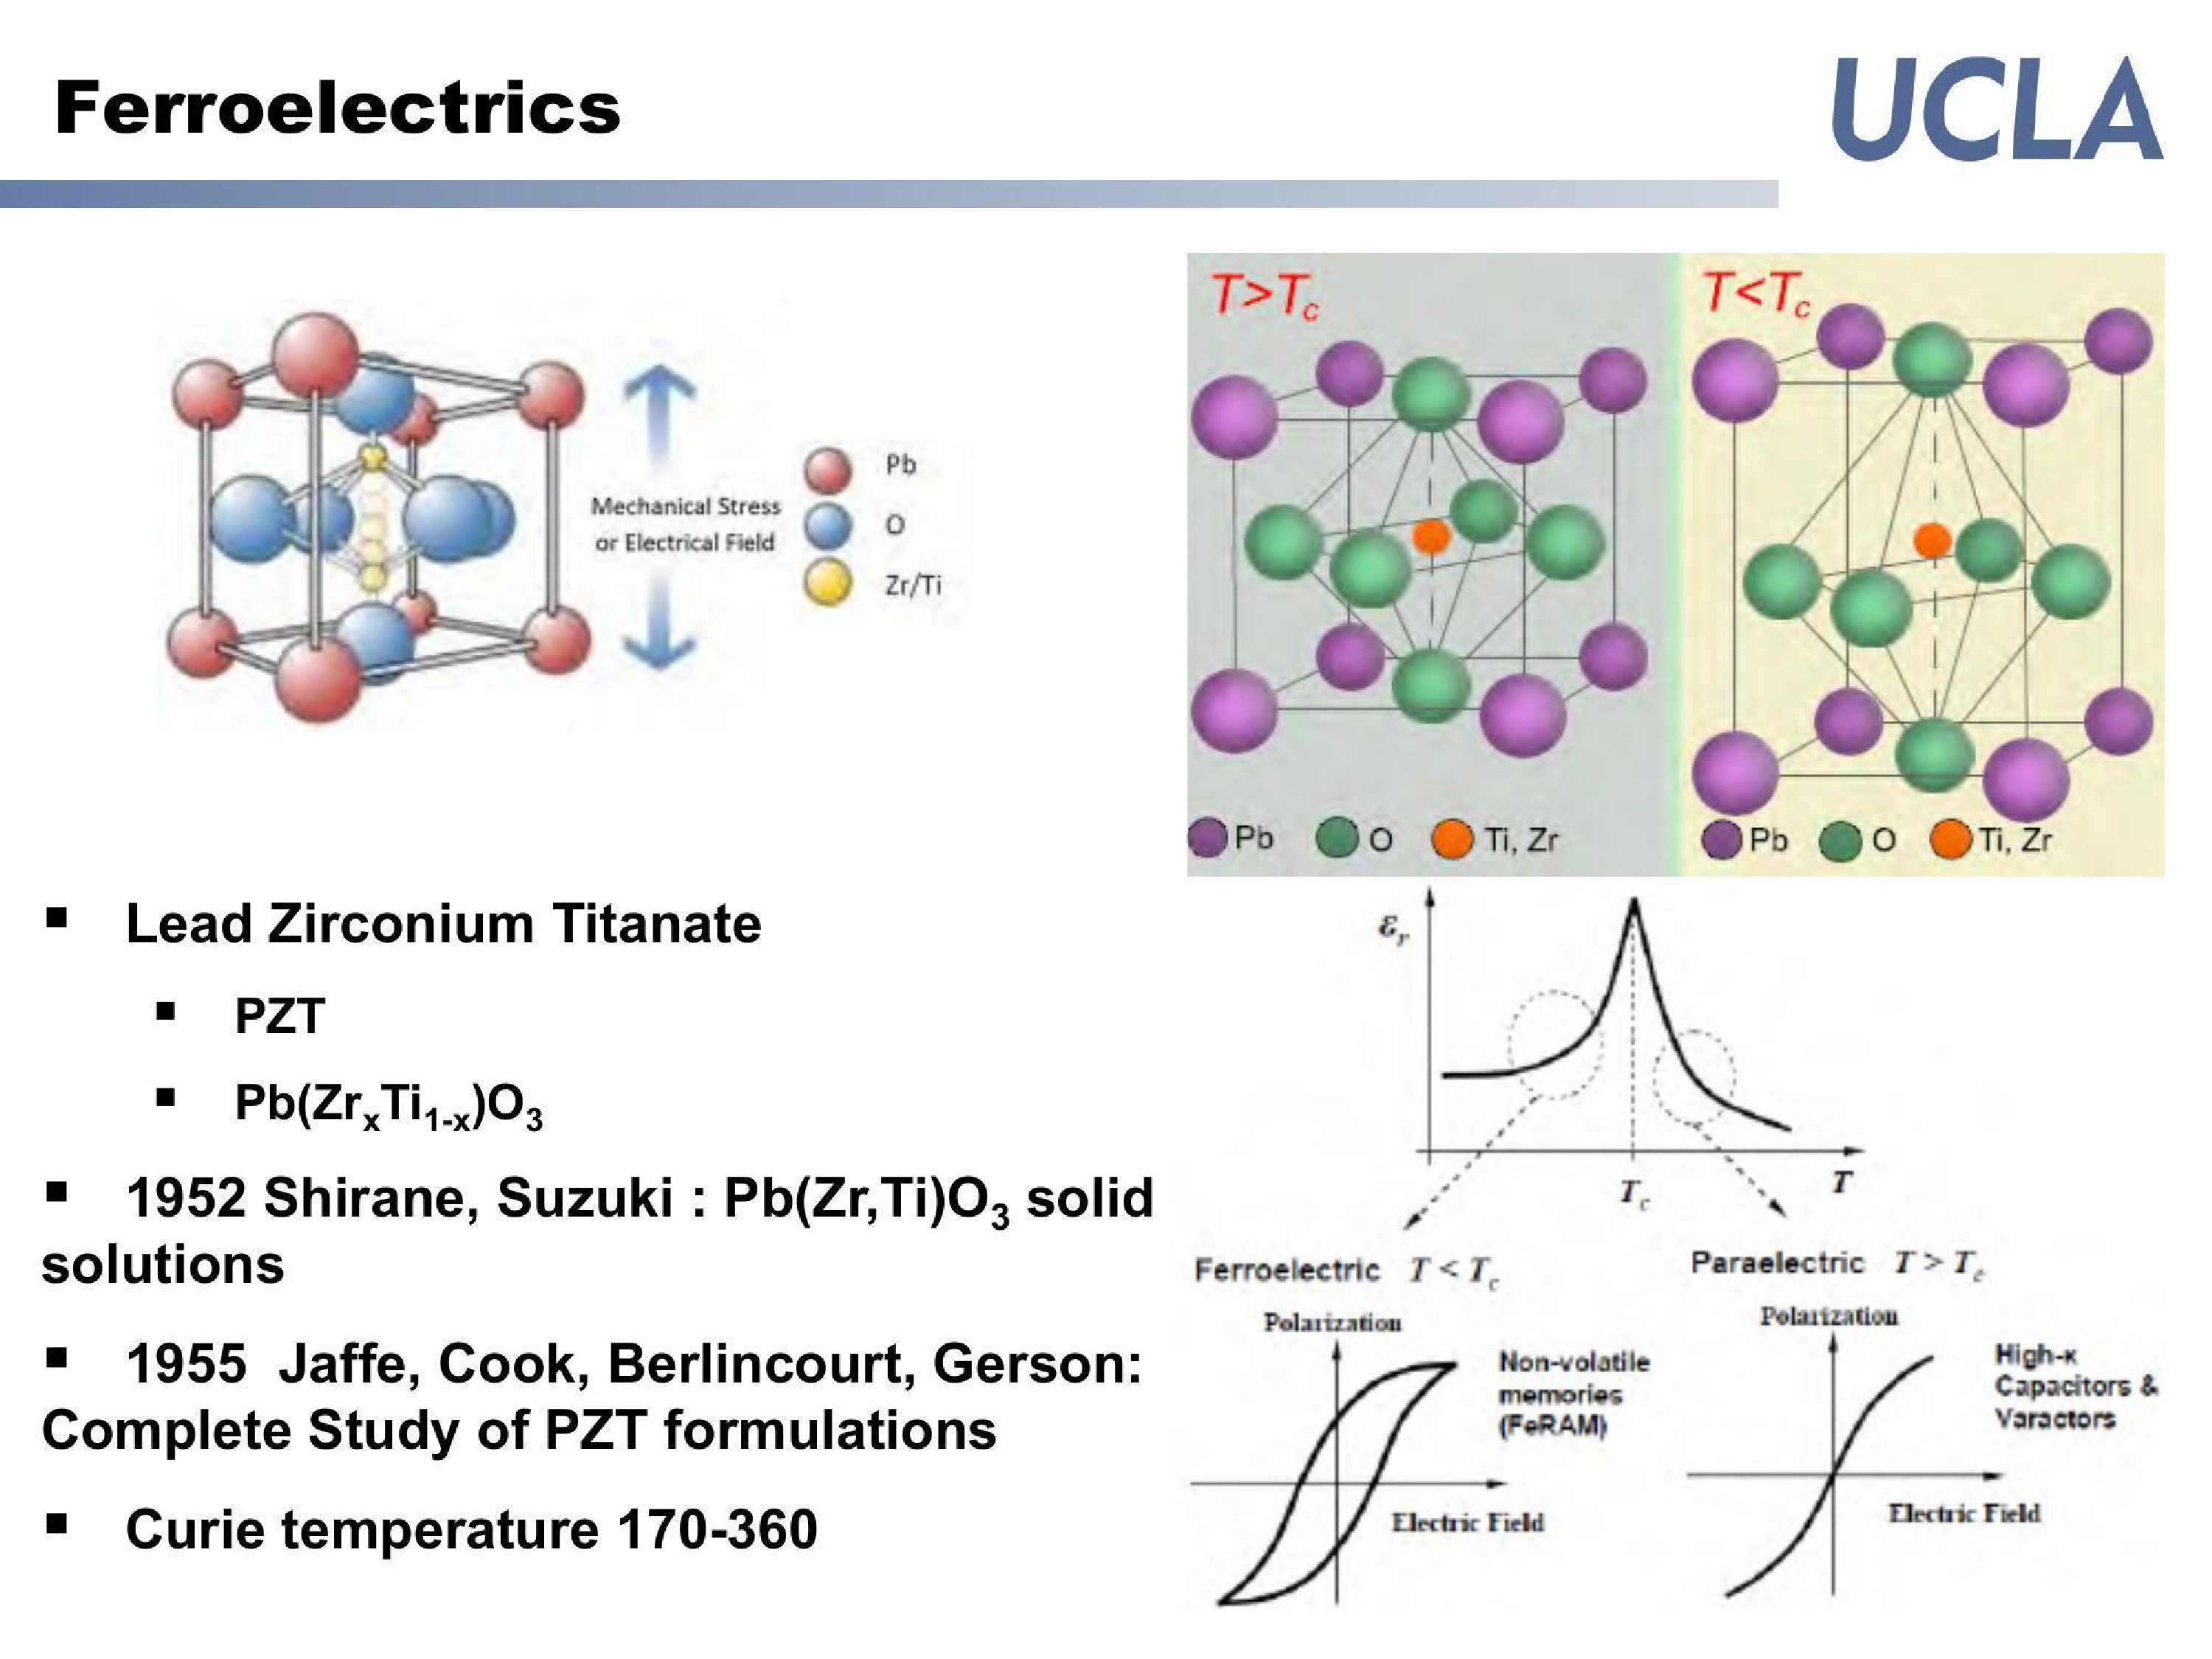
\includegraphics[width=0.8\linewidth,frame]{figures/examples_assests/document_understanding/answer.pdf} \\
\hline
\end{tabular}
\caption{\textbf{Example of a Document Understanding task from Vidore Benchmark, dataset \emph{SyntheticDOCQA healthcare industry BEIR}.}}
\label{fig:doc_understanding_example}
\end{figure}